%*****************************************************************************
%
% Filename : Layered_to_grid.tex
%
% Function : Show how to generate a grid model from a layered model
%
% Author : XingzhongLi
%
% Date : 2018/11
%
%*****************************************************************************

\documentclass[12pt, a4paper]{article}

% packages :
\usepackage{indentfirst}
\usepackage{amsmath}
\usepackage{graphicx}
\graphicspath{{Figures/}}
\usepackage[colorlinks, linkcolor = blue]{hyperref}
\usepackage{hyperref}
\hypersetup{colorlinks,
    linkcolor = blue,
    filecolor = black,
    urlcolor = blue,
    citecolor = blue,
    pdftitle = {For Alstom},
    pdfauthor = {           },
    pdfsubject = {          },
    pdfkeywords = {         },
    pdfproducer = {ps2pdf}
}

% title :
\title{\textbf{\Huge Layered To Grid}}
\author{\textbf{XingzhongLi}\thanks{Email : xzli8@mail.ustc.edu.cn}}
\date{\textbf{\today}}

\begin{document}
\maketitle

\newpage
\tableofcontents

\newpage
\section{Introduction}
%********************************************************************************************
%
% Filename : 01_Introduction.tex
%
% Function : Introduction
%
% Author : XingzhongLi
%
% Date : 2018/11
%
%********************************************************************************************

In the field of geophysics, especially in seismology, we usually want to get a grid model 
to do our calculation on it. But there is no ready-made grid model, we have to generate 
the grid model from other models. For example, there are many layered models in nature. 
So how to generate a grid model from a layered model is our problem. \par

As shown in Figure \ref{fig:Layered_model}, a typical layered model, with two undulating 
interfaces. And each layer has a P wave velocity : 4.0 km/s in the first layer, 5.0 km/s 
in the second layer and 6.0 km/s in the third layer.
\begin{figure}[h]
    \begin{center}
        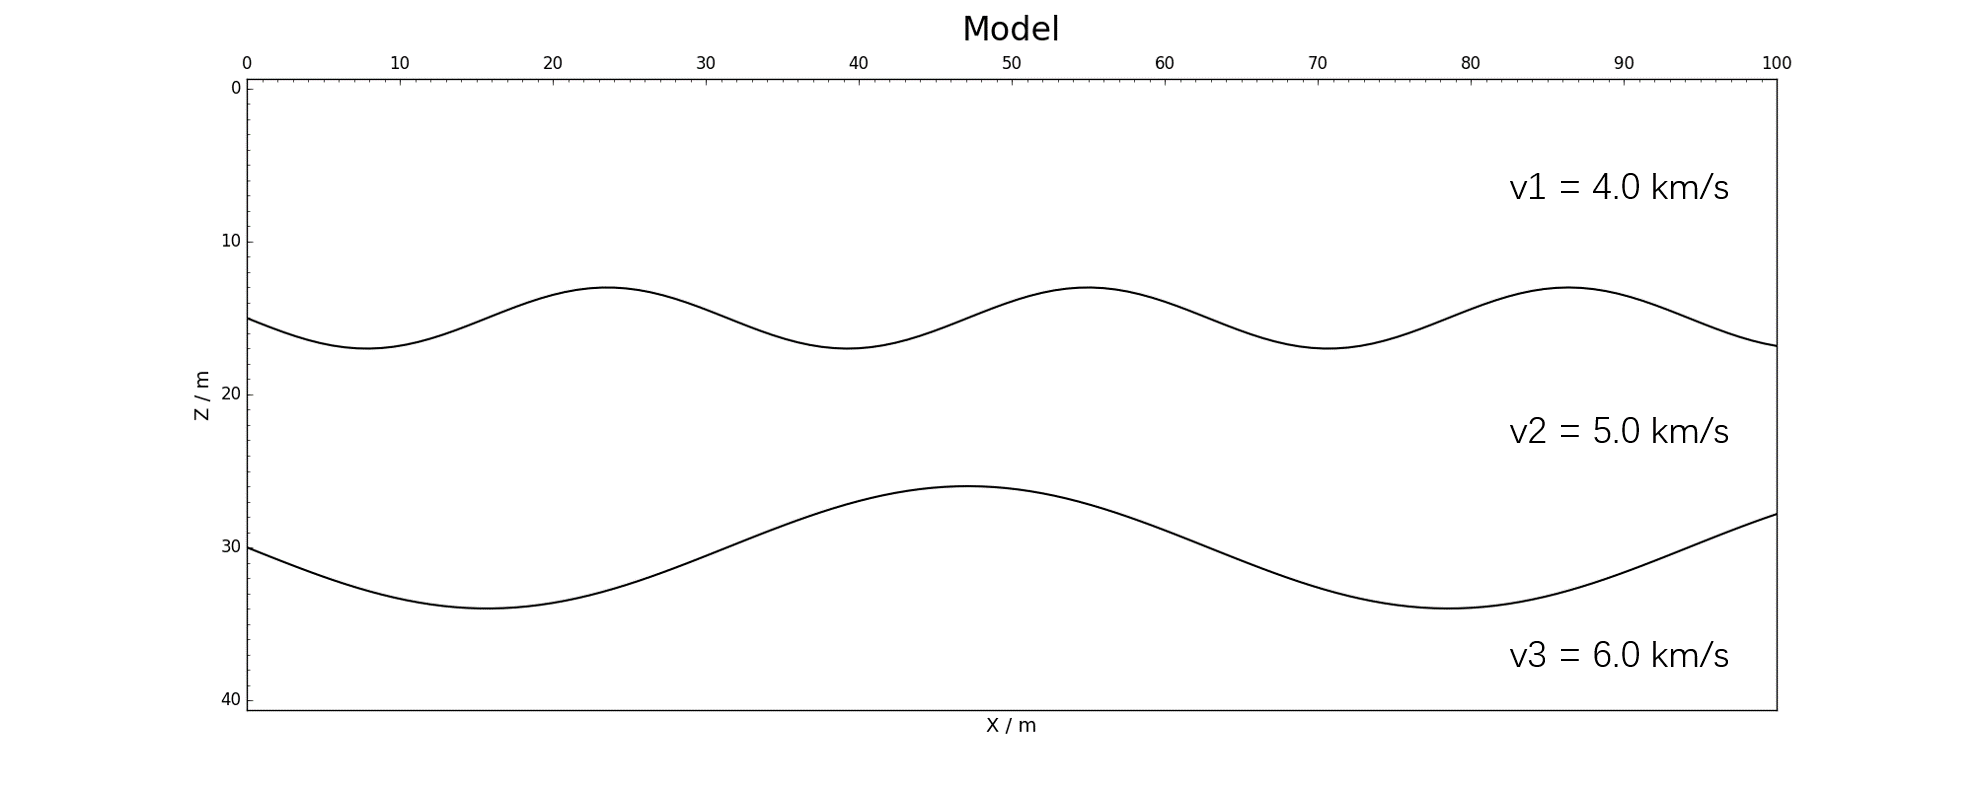
\includegraphics[scale = 0.35]{Layered_model.png}
    \end{center}
    \label{fig:Layered_model}
    \caption{Layered model}
\end{figure}

The grid we want to get from the layered model is shown in Figure \ref{fig:Grid} :
\begin{figure}[h]
    \begin{center}
        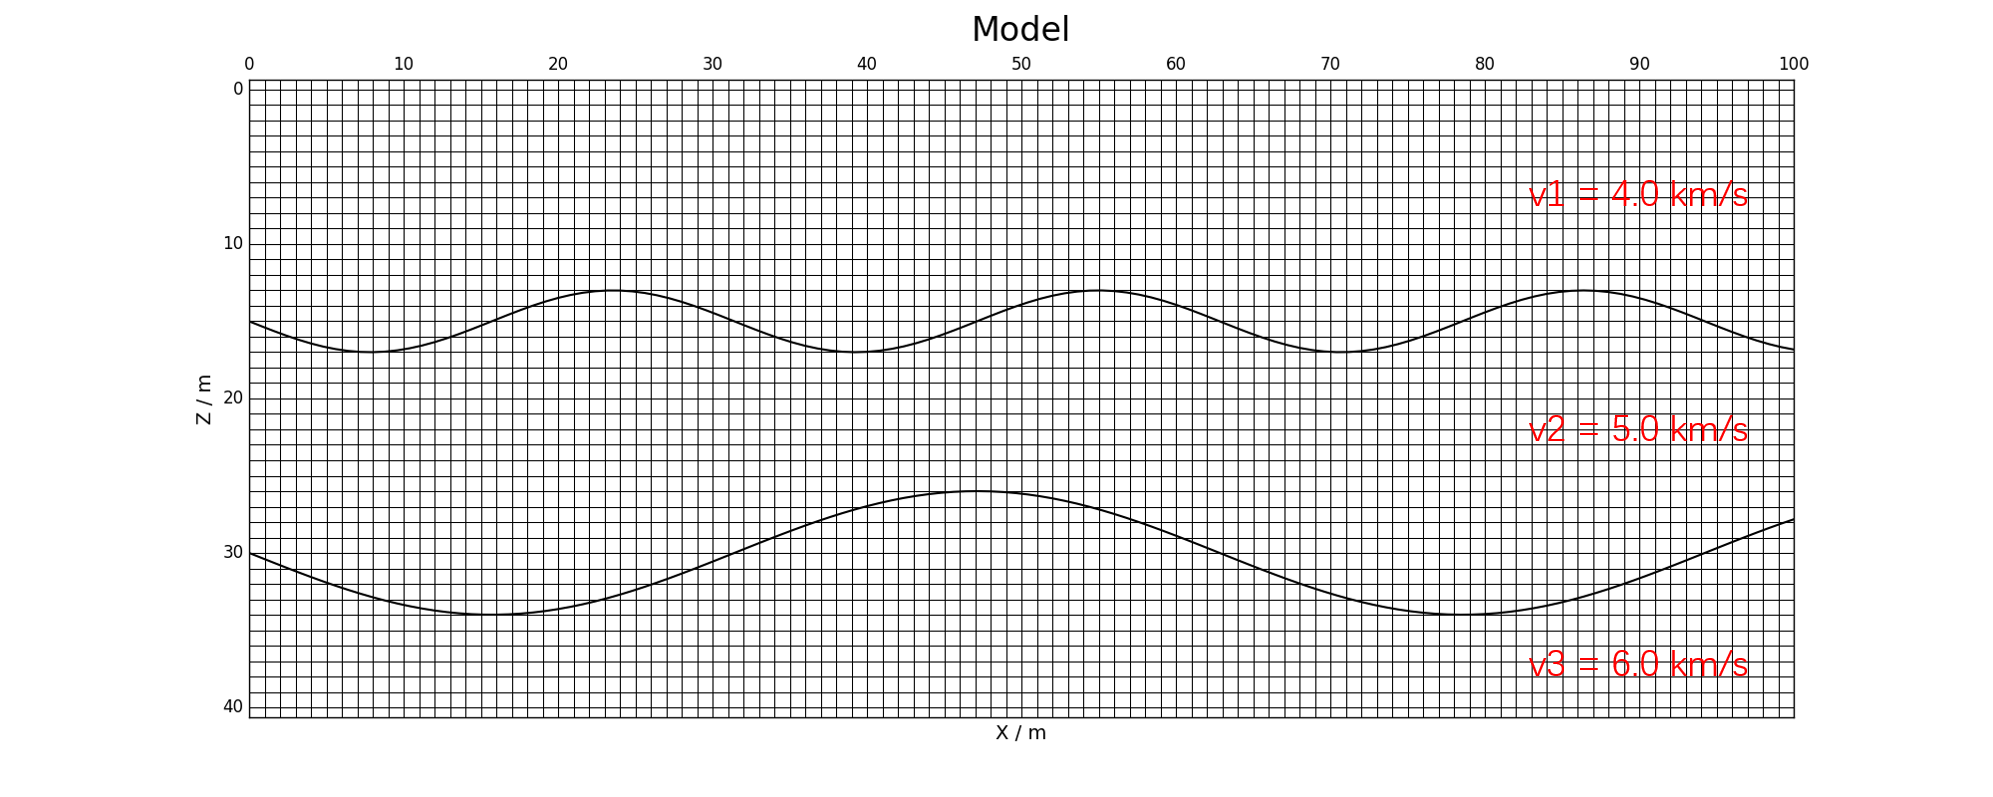
\includegraphics[scale = 0.35]{Grid.png}
    \end{center}
    \label{fig:Grid}
    \caption{Grid}
\end{figure}


\newpage
\section{Method}
%********************************************************************************************
%
% Filename : 02_Method.tex
%
% Function : Method
%
% Author : XingzhongLi
%
% Date : 2018/11
%
%********************************************************************************************

\subsection{Input the information of grid and layer}
In order to generate the grid model, we must know some information about the grid model. 
First of all, the range of the grid model must be given, in other words, we must know the 
minimum and maximum value of x and z coordinate of the 2D grid model, we name them as 
``xmin'', ``xmax'', ``zmin'', ``zmax'' respectively. Only the information of range is not 
enough to generate the grid, we still need to know the grid spacing ``d\_grid''. These is 
all the information about the grid model and they should be stored in the file named 
``grid.dat'' which is in the directory ``input/''. The grid information is input through 
the function ``input\_grid'' which is included in the module ``mod\_io.py''.\par

Besides, we also need to know some information about the interfaces, which is the most 
important thing in this case. Firstly, the number of layer must be given, we named it as 
``num\_layer''. The next is the spacing between every two interface nodes, because the shape 
of the interface is described by a series of discrete nodes, we name it as ''d\_layer''.
The velocity of each layer also should be given, we name it as ``v\_layer'', and this parameter
should be a list or an array in our python codes because there maybe several layers inside
the 2D model. The last, also the most important, is the depth of the discrete interface nodes,
also the z coordinate of each node. This information can be get by actually measurement and
also can be get by synthesis. For example, it can be synthesized by a function, and a 
function based on ``sin'' is chosen here. The expression of the function is : \par
\begin{align}
    z = A sin(\omega x) + z_0
\end{align}
The parameter ``$A$'' means the amplitude of ``sin'', so it is referred to as 
''amplitude\_layer''. ``$\omega$'' means the angular frequency of ``sin'', so it is went
the name of ``w\_layer''. ``$z_0$'' means the starting depth of ``sin'', so it is called
``depth\_layer''. All of them are list or array in our python codes and they are stored in
the file ``layer.dat'' included in the directory ``input/''. These information is input
through the function ``input\_layer'' which is included in the module ``mod\_io.py''. \\[5pt]

\subsection{How to generate the undulating interface}
\indent In order to get an undulating interface, we use the function based on ``sin'' mentioned 
above to calculate x and z coordinate of the discrete nodes on the interface, but in fact 
the coordinate information of the interface is obtained through other means, such as measured.
If you want to get an interface with other forms, you can change the function based on ``sin''
to whatever you want. The achievement of the function based on ``sin'' is put in the function 
named "generate\_layer" contained in the file "mod\_layer.py". \\[5pt]

\subsection{How to generate the grid model}
The generation of grid model is based on the interface. According to the z-coordinate of nodes
on interface and the velocity of each layer, we can divide the grid model into several parts,
and each part has a constant velocity. But one problem is that the spacing of grid named
``d\_grid'' maybe different from the spacing of interface nodes named ``d\_layer'', so before
dividing, we have to make the two kinds of nodes matched. The matching tasks are done through
interpolation. For each x-coordinate on grid, we calculate the corresponding z-coordinate of
each interface according to the adjacent two nodes on the interface by linear interpolation.
The achievement of this part has been put in the function called ``layer\_depth'' included in
the module ``mod\_grid.py''. The achievement of generating grid model has been put in the 
function ``generate\_grid'', also in the module ``mod\_grid.py''. \\[5pt]

\subsection{Plot the grid model}
We also provide a function called ``plot\_model'' in the module ''mod\_plot.py'' to plot the
grid model. You can see the codes for more details. \\[5pt]

\subsection{Output the grid model}
The function called ``output\_model'' included in the module ``mod\_io.py'' can output the
information of the grid model to file in a specific format. Because we want to use this grid
model as an input file in our MFMM2D program, so it is output in this format, you can change
the output format as you want by modifying the function ``output\_model''. \\[5pt]



%\newpage
\section{Result}
%********************************************************************************************
%
% Filename : 03_Results.tex
%
% Function : Results
%
% Author : XingzhongLi
%
% Date : 2018/11
%
%********************************************************************************************

The grid model is presented here :
\begin{figure}[h]
    \begin{center}
        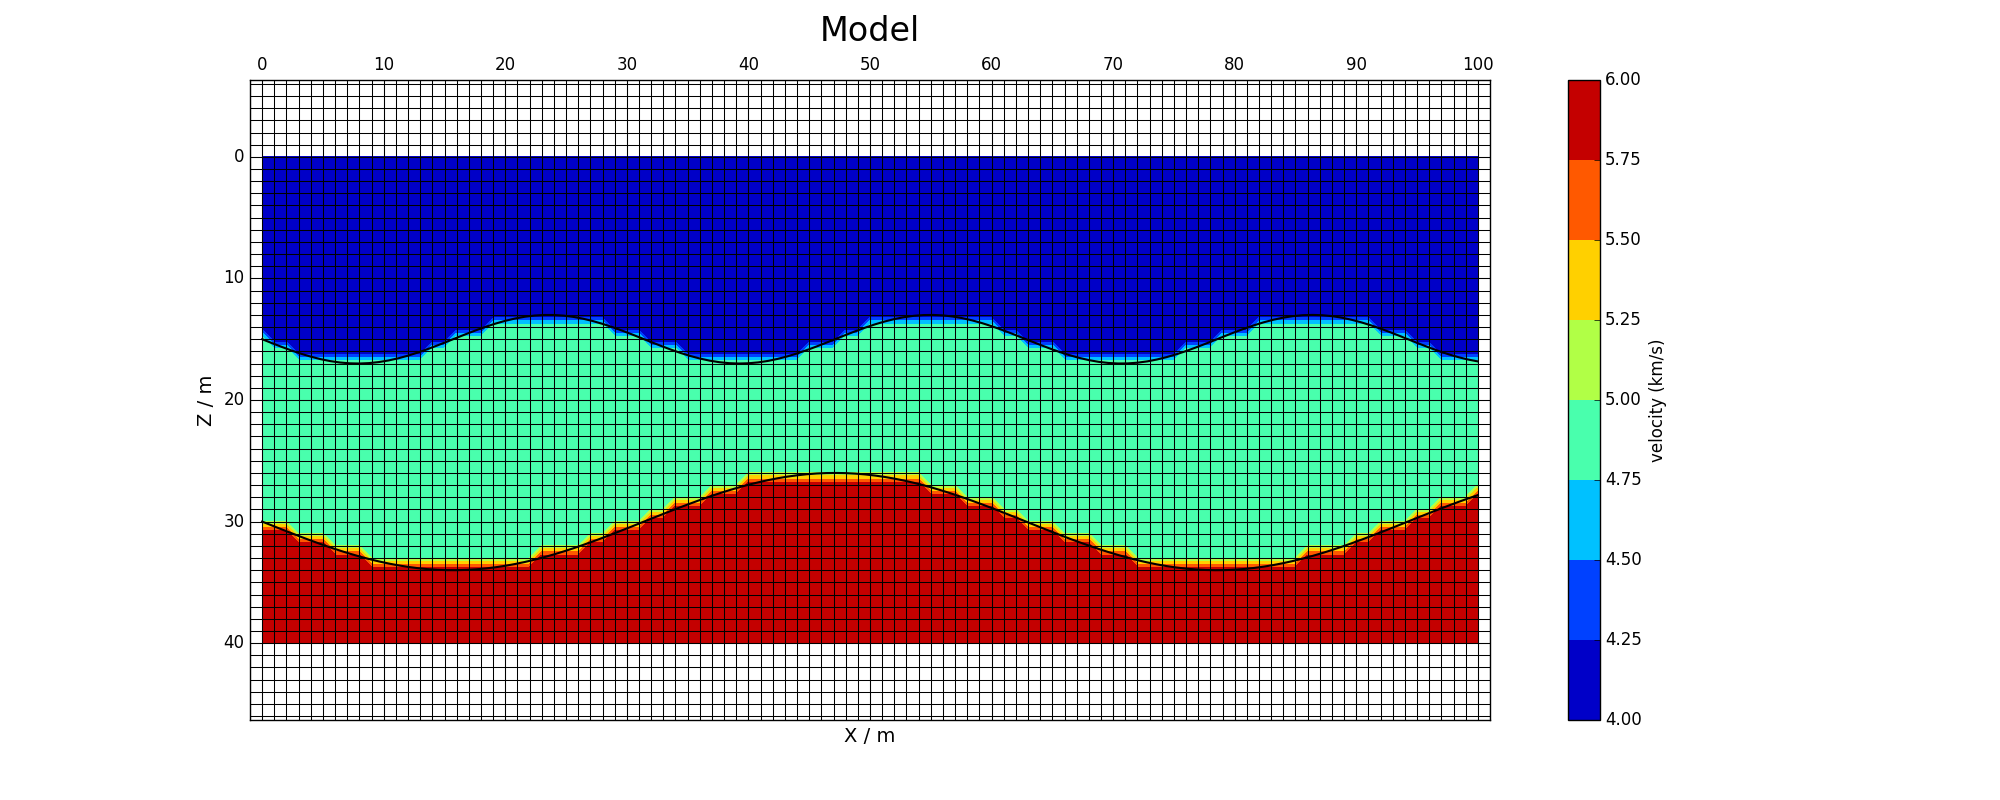
\includegraphics[scale = 0.3]{Grid_model.png}
    \end{center}
    \label{fig:Grid_model}
    \caption{Grid model}
\end{figure}


\newpage
\section{Appendix}
%********************************************************************************************
%
% Filename : 04_Appendix.tex
%
% Function : Appendix
%
% Author : XingzhongLi
%
% Date : 2018/11
%
%********************************************************************************************

1.You can get the python codes on github :
\url{https://github.com/xzli8/Layered\_to\_grid\_2D} \par
2.Please feel free to contact with the author if you have any problem, 
I will try my best to help you.


\end{document}
